\documentclass[
]{jss}

\usepackage[utf8]{inputenc}

\providecommand{\tightlist}{%
  \setlength{\itemsep}{0pt}\setlength{\parskip}{0pt}}

\author{
Carlos Cinelli\\University of California, Los Angeles \And Jeremy Ferwerda\\Dartmouth College \And Chad Hazlett\\University of California, Los Angeles
}
\title{\pkg{sensemakr}: Sensitivity Analysis Tools for OLS}

\Plainauthor{Carlos Cinelli, Jeremy Ferwerda, Chad Hazlett}
\Plaintitle{\pkg{sensemakr}: Sensitivity Analysis Tools for OLS}
\Shorttitle{\pkg{sensemakr}: Sensitivity Analysis Tools for OLS}

\Abstract{
This paper introduces the \proglang{R} and \proglang{Stata} package
\pkg{sensemakr} for assesing the sensitivity of regression estimates to
unobserved confounding. The package provides a suite of tools for
sensitivity analysis in regression models developed in
\citet{cinelli:jrssb2019}. These tools are based on the familiar omitted
variable bias framework, and can be easily computed using only standard
regression results. Furthermore, they do not require assumptions on the
functional form of the treatment assignment mechanism nor on the
distribution of the unobserved confounders, naturally handle multiple
confounders, possibly acting non-linearly, and enable bounding of
sensitivity parameters employing domain knowledge.
}

\Keywords{causal inference, sensitivity analysis, omitted variable bias, robustness value, R, Stata}
\Plainkeywords{causal inference, sensitivity analysis, omitted variable bias, robustness value, R, Stata}

%% publication information
%% \Volume{50}
%% \Issue{9}
%% \Month{June}
%% \Year{2012}
%% \Submitdate{}
%% \Acceptdate{2012-06-04}

\Address{
    Carlos Cinelli\\
  University of California, Los Angeles\\
  Department of Statistics, 8125 Math Sciences Building, Los Angeles, CA
  90095, USA.\\
  E-mail: \email{carloscinelli@ucla.edu}\\
  URL: \url{http://carloscinelli.com}\\~\\
      Jeremy Ferwerda\\
  Dartmouth College\\
  Department of Government, Hanover, NH 03755\\
  E-mail: \email{jeremy.a.ferwerda@dartmouth.edu}\\
  URL: \url{http://jeremyferwerda.com/}\\~\\
      Chad Hazlett\\
  University of California, Los Angeles\\
  Department of Statistics, 8125 Math Sciences Building, Los Angeles, CA
  90095, USA.\\
  E-mail: \email{chazlett@ucla.edu}\\
  URL: \url{http://chadhazlett.com}\\~\\
  }


% Pandoc header

\usepackage{amsmath}

\begin{document}

\hypertarget{intro}{%
\section{Introduction}\label{intro}}

Investigators in a wide range of disciplines face the perennial
challenge of making and defending causal claims using observational
sources of data in which they could not ensure the ``treatment''
variable of interest was randomized or otherwise free of confounding.
The most common identification strategy, in such circumstances, is to
condition on or ``adjust for'' observed covariates in the hopes that
there are not problematic unobserved covariates that remain. Linear
regression remains among the most widely used approaches to realize such
adjustments. However, supporting the claim that the coefficient from
such a regression unbiasedly estimates a causal quantity requires
defending an untestable assumption that there are no unobserved
confounders. Moreover, such an assumption does not need to hold
precisely (and never does) in order for a research result to remain
substantively valid and informative. Sensitivity analyses quantify how
strong unobserved confounding needs to be to change the research
conclusions. They also aid in reasoning as whether confounding of such
strength is plausible. This gives investigators the ability to
rigorously describe the fragility of putative causal estimates in the
face of potential unobserved confounding.

The goal of this paper is to introduce the \proglang{R} and
\proglang{Stata} package \pkg{sensemakr}
\citep{sensemakr:R,sensemakr:stata}, which implements a suite of
sensitivity analysis tools proposed in \citet{cinelli:jrssb2019} for
assessing the sensitivity of a regression coefficient to the inclusion
of omitted variables. The goal of \pkg{sensemakr} is to make it easy to
understand the impact that omitted variables would have on a regression
result. This allows analysts to investigate the robustness of their
estimates to violations of the assumption of no unobserved confounding,
answering questions such as:

\begin{itemize}
\item
  How strong would an unobserved confounder (or a group of confounders)
  have to be to change our research conclusions?
\item
  In a worst-case scenario, how robust are our results to all unobserved
  confounders acting together, possibly non-linearly?
\item
  How strong would confounding need to be relative to the strength of
  observed covariates, to change our answer by a certain amount?
\end{itemize}

Various sensitivity analyses have been proposed dating back to
\citet{cornfield1959smoking}, with more recent contributions including
\citep{rosenbaum1983assessing, robins1999association, frank:smr2000, rosenbaum2002gamma, imbens2003sensitivity, brumback2004sensitivity, frank:eepa2008, hosman2010sensitivity, imai2010identification, arah2011, blackwell2013selection, frank2013would, carnegie:jree2016, dorie2016flexible, middleton2016bias, oster:jbes2017, cinelli:icml2019, franks:jasa2019}.
Yet, such sensitivity analyses remain underutilized. We argue that a
number of factors contribute to this reluctant uptake. One is the
complicated nature and strong assumptions many of these methods impose,
sometimes involving restrictions on or even a complete description of
the nature of the confounder. A second reason is that though users
routinely report ``regression tables'' (or perhaps coefficient plots) to
convey the results of a regression, until recently we have lacked
``standard'' quantities that can simply and correctly summarize
sensitivity in the face of unobserved confounding. Third, and most
fundamentally, connecting the results of a formal sensitivity analysis
to a cogent argument about what types of confounders may exist in one's
research project is often difficult, particularly when there are no
compelling arguments as to why the treatment assignment should be
approximately ``ignorable'', ``exogeneous'', or ``as-if random''.
Further, some of the solutions offered by the literature can lead users
to erroneous conclusions.

This paper is organized as follows. Section \ref{review} briefly reviews
the omitted variable bias framework for sensitivity sensitivity analysis
proposed in \citet{cinelli:jrssb2019}; this framework provides the
theoretical foundations for the tools developed in \pkg{sensemakr}.
Next, Section \ref{r-basic} goes over the the basic functionality and
provides a practical introduction to sensitivity analysis using
\proglang{sensemakr} for \proglang{R}. Section \ref{r-adv} looks at
advanced usage of the \proglang{R} package, and shows how to leverage
individual functions for customized sensitivity analyses. Finally,
Section \ref{stata} describes \proglang{sensemakr} for \proglang{Stata}.
We end the paper with final remarks\ldots{}

\hypertarget{review}{%
\section{Sensitivity analysis in an omitted variable bias
framework}\label{review}}

In this section, we briefly review the omitted variable bias (OVB)
framework for sensitivity analysis presented in
\citet{cinelli:jrssb2019}. This method builds on a scale-free
reparameterization of the OVB formula in terms of partial \(R^2\)
values. Benefits of the parameterization include:

\begin{itemize}
\tightlist
\item
  assessing the sensitivity of multiple confounders acting together,
  possibly non-linearly;
\item
  assessing the sensitivity to extreme scenarios in which all (or a
  designated portion) of the residual variation of the oucome is assumed
  to be explained by unobserved confounding;
\item
  exploiting knowledge of relative strength of variables to bound the
  bias due to unobserved confounding;
\item
  presenting all sensitivity results concisely, for easy routine
  reporting.
\end{itemize}

\hypertarget{ovb}{%
\subsection{The OVB framework}\label{ovb}}

The starting point of our analysis is a \emph{full} (or ``long'') linear
regression model of an outcome \(Y\) on a treatment \(D\), controlling
for a set of covariates given by \emph{both} \({\bf X}\) and \(Z\),
\begin{align}
Y &= \hat{\tau} D + {\bf X} \hat{{\bf \beta}} +  \hat{\gamma}Z + \hat{\epsilon}_{\text{full}}  \label{eq:fulleq}
\end{align} \noindent where \(Y\) is an \((n \times 1)\) vector
containing the outcome of interest for each of the \(n\) observations
and \(D\) is an \((n \times 1)\) treatment variable (which may be
continuous or binary); \({\bf X}\) is an \((n \times p)\) matrix of
\emph{observed} covariates including the constant; and \(Z\) is a single
\((n \times 1)\) \emph{unobserved} covariate (we discuss how to extend
results for a multivariate \(Z\) below).

Equation \ref{eq:fulleq} is the regresion model that the investigator
\emph{wished} she had run to obtain a valid causal estimate of the
effect of \(D\) on \(Y\). Nevertheless, \(Z\) is unobserved. Therefore,
the feasible regression the investigator is able to estimate is the
\emph{restricted} (or ``short'') model \emph{omitting} \(Z\), that is,
\begin{align}
Y  &= \hat{\tau}_{\text{res}} D + {\bf X} \hat{{\bf \beta}}_{\text{res}} + \hat{\epsilon}_{\text{res}}\label{eq:restrictedeq}
\end{align}

Given the discrepancy of what we wish to know and what we actually have,
the main question we would like to answer is: how do the observed point
estimate and standard error of the restricted regression,
\(\hat{\tau}_{\text{res}}\) and
\(\widehat{se}(\hat{\tau}_{\text{res}})\), compare to the desired point
estimate and standard error of the full regression, \(\hat{\tau}\) and
\(\widehat{se}(\hat{\tau})\)?

\hypertarget{ovb-with-the-partial-r2-parameterization}{%
\subsubsection{OVB with the partial R2
parameterization}\label{ovb-with-the-partial-r2-parameterization}}

Define as \(\widehat{\text{bias}}\) the difference between the full and
restricted estimates,

\begin{align}
\widehat{\text{bias}}~:=~\hat{\tau}_{\text{\text{res}}}~-~\hat{\tau}
\end{align}

Now let: (i) \(R^2_{D\sim Z | {\bf X}}\) denote the share of residual
variance of the \emph{treatment} \(D\) explained by the omitted variable
\(Z\), after accounting for the remaining covariates \({\bf X}\); and,
(ii) \(R^2_{Y\sim Z|D, {\bf X}}\) denote the share of residual variance
of the \emph{outcome} \(Y\) explained by the omitted variable \(Z\),
after accounting for \({\bf X}\) and \(D\). \citet{cinelli:jrssb2019}
have shown that these quantities are sufficient for determining the
bias, adjusted estimate and adjusted standard errors of the full
regression of Equation \ref{eq:fulleq}.

More precisely, the bias can be written as,

\begin{align}
|\widehat{\text{bias}}| &= \widehat{\text{se}}(\hat{\tau}_{\text{res}}) \sqrt{\frac{ R^2_{Y\sim Z|D, {\bf X}}~ R^2_{D\sim Z | {\bf X}}}{1 - R^2_{D\sim Z | {\bf X}}} (\text{df})} \label{eq:r2bias2}
\end{align}

Where \(\text{df}\) stands for the degrees of freedom of the restricted
regression actually run. Moreover, the estimated standard error of
\(\hat{\tau}\) can be recoverd with,

\begin{align}
\widehat{\text{se}}(\hat{\tau})  = \widehat{\text{se}}(\hat{\tau}_{\text{res}}) \sqrt{\frac{1 - R^2_{Y\sim Z|D, {\bf X}}}{1 - R^2_{D\sim Z | {\bf X}}} \left(\frac{\text{df}}{\text{df}-1}\right)}.  \label{eq:r2se} 
\end{align}

Given hypothetical values of \(R^2_{D\sim Z | {\bf X}}\) and
\(R^2_{Y\sim Z|D, {\bf X}}\), Equations \ref{eq:r2bias2} and
\ref{eq:r2se} allow investigators to examine the sensitivity of point
estimates and standard-errors (and consequently also t-values,
confidence intervals or p-values) to the inclusion of any omitted
variable \(Z\) with such strengths. Or, coversely, given a critical
threshold deemed to be problematic, one can find the strength of
confounders capable of bringing about a bias of that ammount. Another
useful property of the OVB formula with the partial \(R^2\)
parameterization is that the effect of \(R^2_{Y\sim Z|D, {\bf X}}\) on
the bias is bounded. This allows investigators to contemplate extreme
sensitivity scenarios, in which the parameter
\(R^2_{Y\sim Z|D, {\bf X}}\) is set to 1 (or another conservativie
value), and see what happens as \(R^2_{D\sim Z | {\bf X}}\) varies.

\hypertarget{rv-and-r2yd}{%
\subsection{Sensitivity statistics for routine
reporting}\label{rv-and-r2yd}}

The previous formulas fully determine the bias (or adjusted values) of
the estimate and the standard error for any given degree of confounding,
and as such can be used in numerous ways to explore the sensitivity of a
regression result. For instance, sensitivity contour plots and
sensitivity plots of extreme scenarios, which we demonstrate in the next
sections using \pkg{sensemakr}, allow us to fully explore the
sensitivity of an estimate as we vary both sensitivity parameters.

Nevertheless, making sensitivity analysis standard practice benefits
from simple and interpretable statistics which can quickly describe the
sensitivity of a study to unobserved confounding. These statistics serve
two main purposes:

\begin{enumerate}
\def\labelenumi{\arabic{enumi}.}
\item
  They can be easily displayed alongside other usual summary statistics
  in regression tables, making a minimal sensitivity analysis to
  unobserved confounding simple, accessible and standardized;
\item
  They can be easily computed from quantities found in a rregression
  table, thereby enabling readers and reviwers to assess the sensitivity
  of results they see in print, even if the original authors did not
  perform sensitivity analyses.
\end{enumerate}

With this in mind, \citet{cinelli:jrssb2019} propose two main
sensitivity statistics for \emph{routine reporting}: (i) the (observed)
partial \(R^2\) of the treatment with the outcome,
\(R^2_{Y\sim D \mid {\bf X}}\); and, the \emph{robustness value}.

\hypertarget{the-partial-r2-of-the-treatment-with-the-outcome}{%
\subsubsection{The partial R2 of the treatment with the
outcome}\label{the-partial-r2-of-the-treatment-with-the-outcome}}

Beyond being an effect measure that quantifies how much variation of the
outcome the treatment explains, the partial \(R^2\) of the treatment
with the outcome can also be used to convey how robust the point
estimate is to unobserved confounding in an ``extreme scenario.'' More
precisely, suppose the unobserved confounder \(Z\) explains \emph{all}
residual variance of the outcome, that is,
\(R_{Y\sim Z|D, {\bf X}}~=~1\). Then, for this confounder to bring the
point estimate to zero, it must explain \emph{at least} as much residual
variation of the treatment as the residual variation of the outcome that
the treatment currently explains. In other words, if
\(R_{Y\sim Z|D, {\bf X}}~=~1\), then we must have that
\(R^2_{D\sim Z|{\bf X}} \geq R^2_{Y\sim D|{\bf X}}\), otherwise this
confounder cannot logically account for all the observed association
between the treatment and the outcome \citep{cinelli:jrssb2019}.

\hypertarget{the-robustness-value}{%
\subsubsection{The Robustness Value}\label{the-robustness-value}}

The second sensitivity statistics proposed in \citet{cinelli:jrssb2019}
is the \emph{robustness value}. The robustness value \(RV_{q,\alpha}\)
quantifies the \emph{minimal} strength of association that the
confounder needs to have, \emph{both} with the treatment and with the
outcome, so that a confidence interval of level \(\alpha\) includes a
change of \(q\%\) of the current estimated value.

Let \(f_q := q|f_{Y\sim D | {\bf X}}|\), where
\(|f_{Y\sim D | {\bf X}}|\) is the partial \emph{Cohen's f} of the
treatment with the outcome multiplied by the percentage reduction \(q\)
deemed to be
problematic.\footnote{Cohen's $f^2$ can be written as $f^2_{Y\sim D | {\bf X}} = R^2_{Y\sim D | {\bf X}}/(1-R^2_{Y\sim D | {\bf X}})$}
Also, let \(|t^*_{\alpha, \text{df}-1}|\) denote the t-value threshold
for a t-test with significance level of \(\alpha\) and \(\text{df}-1\)
degrees of freedom, and define
\(f^*_{\alpha, \text{df} - 1} := |t^*_{\alpha, \text{df}-1}|/\sqrt{\text{df} -1}\).
Finally, construct \(f_{q, \alpha}\), which ``deducts'' from
\(f_{Y\sim D | {\bf X}}\) both the proportion of reduction \(q\) of the
point estimate and the boundary below which statistical significance is
lost at the level of \(\alpha\). That is,
\(f_{q, \alpha} := f_q - f^*_{\alpha,\text{df} - 1}\). We then have that
\(RV_{q,\alpha}\) is given by \citep{cinelli:jrssb2019, cinelli:wp2020},

\noindent  \begin{align}
RV_{q, \alpha} =\left\{
\arraycolsep=2pt\def\arraystretch{2}
\begin{array}{ll}
\displaystyle 0, & \text{if}~~f_{q, \alpha} < 0 \\
\displaystyle \frac{1}{2}\left(\sqrt{f_{q, \alpha}^4 + 4f_{q, \alpha}^2} - f_{q, \alpha}^2\right), & \text{if}~~ f_{q} < 1/f^*_{\alpha, \text{df}-1}\\
\displaystyle \frac{f_{q}^2 - f^{*2}_{\alpha,\text{df} - 1}}{1+f^2_{q}}, & \text{otherwise}. 
\end{array}\right.
\label{eq:rvt_main}
\end{align}

\noindent Any confounder that explains \(RV_{q,\alpha}\%\) of the
residual variance \emph{both} of the treatment and of the outcome is
sufficiently strong to make the adjusted t-test not reject the null
hypothesis \(H_0: \tau = (1-q)|\hat{\tau}_{\text{res}}|\) at the
\(\alpha\) level (or, equivalently, sufficiently strong to make the
adjusted \(1-\alpha\) confidence interval include
\((1-q)|\hat{\tau}_{\text{res}}|\)). Likewise, a confounder with both
associations lower than \(RV_{q, \alpha}\) is not capable of overturning
the conclusion of such a test. Setting \(\alpha =1\) returns the
robustness value for the point estimate. Further details on how to
interpret the RV in practice are given in the next sections.

\hypertarget{bounds}{%
\subsection{Bounds on the strength of confounding using observed
covariates}\label{bounds}}

Consider a confounder orthogonal to the observed covariates, ie.,
\(Z \perp {\bf X}\), or, equivalently, consider only the part of \(Z\)
not linearly explained by \({\bf X}\). Now denote by \(X_j\) a specific
covariate of the set \({\bf X}\) and define

\noindent  \begin{align}
k_D := \frac{R^2_{D\sim Z|{\bf X}_{-j}}}{R^2_{D\sim X_{j}|{\bf X}_{-j}} },  \qquad k_Y := \frac{R^2_{Y \sim Z |{\bf X}_{-j},D}}{R^2_{Y \sim X_{j} |{\bf X}_{-j},D}}.
\end{align}

where \({\bf X}_{-j}\) represents the vector of covariates \({\bf X}\)
excluding \(X_{j}\). That is, the terms \(k_D\) and \(k_Y\) represent
how strong the confounder \(Z\) is relative to observed covariate
\(X_j\), where ``strength'' is measured by how much residual variation
they explain of the treatment (for \(k_D\)) and of the outcome (for
\(k_Y\)). Given \(k_D\) and \(k_Y\), we can rewrite the strength of the
confounders as \citep{cinelli:jrssb2019}, \begin{align}
R^2_{D\sim Z|{\bf X}} = k_D f^2_{D\sim X_{j}|{\bf X}{-j}}, \qquad R^2_{Y\sim Z|D, {\bf X}} \leq \eta^2 f^2_{Y \sim X_j|{\bf X}_{-j},D} \label{eq:bounds}
\end{align}

\noindent where \(\eta\) is a scalar which depends on \(k_Y\), \(k_D\)
and \(R^2_{D\sim X_{j}|{\bf X}{-j}}\).

These equations allow the investigator to assess the maximum bias that a
hypothetical confounder at most ``k times'' as strong as a particular
covariate \(X_j\) could cause. This can be used to explore the relative
strength of confounding necessary for bias to have been problematic and
change the research conclusions. Furthermore, when the researcher has
domain knowledge to argue that a certain covariate \(X_j\) is
particularly important in explaining treatment or outcome variation, and
that omitted variables cannot explain as much residual variance of \(D\)
or \(Y\) as that observed covariate, these results can be used to set
plausible bounds in the total amount of confonding.

\hypertarget{multiple}{%
\subsection{Multiple or non-linear confounders}\label{multiple}}

Finally, suppose that, instead of a single unobserved confounder \(Z\),
there are \emph{multiple} unobserved confounders
\({\bf Z} = [Z_1, Z_2, \dots, Z_k]\). In this case, the regression the
investigator wished she had run becomes,

\noindent  \begin{align}
Y &= \hat{\tau} D + {\bf X} \hat{{\bf \beta}} +  {\bf Z}\hat{{\bf \gamma}} + \hat{\epsilon}_{\text{full}}.  \label{eq:fulleq2}
\end{align}

As \citet{cinelli:jrssb2019} show, the previous results considering a
single unobserved confounder are in fact \emph{conservative} when
considering the impact of multiple confounders, barring an adjustment in
the degrees of freedom of Equation \ref{eq:r2se}. Moreover, since the
vector \({\bf Z}\) is arbitrary, this can also acommodate non-linear
confounders or even misspecification of the functional form of the
observed covariates \({\bf X}\). In other words, to assess the maximum
bias that multiple, non-linear confounders could cause in our current
estimates, it suffices to think in terms of the
\emph{maximum explantory power} that \({\bf Z}\) could have have in the
treatment and outcome regressions, as parameterized by
\(R^2_{D\sim {\bf Z} | {\bf X}}\) and
\(R^2_{Y\sim {\bf Z} |D, {\bf X}}\).

\hypertarget{r-basic}{%
\section{sensemakr for R: basic functionality}\label{r-basic}}

In this section we illustrate the basic functionality of \pkg{sensemkar}
for \proglang{R}. Given that sensitivity analysis requires contextual
knowledge to be properly interpreted, we illustrate these tools with a
real example. We use \pkg{sensemakr} to reproduce all results found in
Section 5 of \citet{cinelli:jrssb2019}, which estimates the effects of
exposure to violence on attitudes towards peace, in Darfur. Further
details about this application and the data can be found in
\citet{hazlett:jcr2019}.

\hypertarget{darfur}{%
\subsection{Violence in Darfur: data and research
question}\label{darfur}}

In 2003 and 2004, the Darfurian government orchestrated a horrific
campaign of violence against civilians, killing an estimated two hundred
thousand people. This application asks whether, on average, being
directly injured or maimed in this episode made individuals more likely
to feel ``vengeful'' and unwilling to make peace with those who
perpetrated this violence. Or, might those who directly suffered such
violence be motivated to see it end, supporting calls for peace?

The \texttt{sensemakr} package provides the data required for this
example based on a survey among Darfurian refugees in eastern Chad
\citep{hazlett:jcr2019}. To get started we first need to install the
package. From within \proglang{R}, the \pkg{sensemakr} package can be
installed from the Comprehensive \proglang{R} Archive Network (CRAN).

\begin{CodeChunk}

\begin{CodeInput}
R> install.packages("sensemakr")
\end{CodeInput}
\end{CodeChunk}

Next, after loading the package, the data can be loaded with the command
\texttt{data("darfur")}.

\begin{CodeChunk}

\begin{CodeInput}
R> library(sensemakr)
R> data("darfur")
\end{CodeInput}
\end{CodeChunk}

The ``treatment'' variable of interest is \texttt{directlyharmed}, which
indicates whether the individual was physically injured or maimed during
the attack on her or his village in Darfur. The main outcome of interest
is \texttt{peacefactor}, an index measuring pro-peace attitudes. Other
covariates in the data include: \texttt{village} (a factor variable
indicating the original village of the respondent), \texttt{female} (a
binary indicator of gender), \texttt{age}, \texttt{herder\_dar} (whether
they were a herder in Darfur), \texttt{farmer\_dar} (whether they were a
farmer in Darfur), and \texttt{past\_voted} (whether they report having
voted in an earlier election, prior to the conflict). For further
details, see \texttt{?darfur}.

\citet{hazlett:jcr2019} argues that the purpose of these attacks was to
punish civilians from ethnic groups presumed to support the opposition
and to kill or drive these groups out so as to reduce this support.
Violence against civilians included aerial bombardments by the
government as well as assaults by the \emph{Janjaweed}, a pro-government
militia. For this example, suppose a researcher argues that, while some
villages were more or less intensively attacked, within village violence
was largely indiscriminate. The bombings could not be finely targeted
owing to their crudeness, and there were not many reason to target them.
Similarly, the \emph{Janjaweed} had no reason to target certain
individuals rather than others, and no information with which to do
so---with one major exception: women were targeted and often subjected
to sexual violence.

Given these considerations, this researcher may argue that adjusting for
\texttt{village} and \texttt{female} is sufficient for control of
confounding, and run the following linear regression model (in which
other pre-treatment covariates, although not necessary for
identification, are also included):

\begin{CodeChunk}

\begin{CodeInput}
R> darfur.model <- lm(peacefactor ~ directlyharmed  + village +  female +
R+                                  age + farmer_dar + herder_dar + 
R+                                  pastvoted + hhsize_darfur, 
R+                    data = darfur)
\end{CodeInput}
\end{CodeChunk}

This regression model results in the estimates shown in Table
\ref{tab:darfur_ols}. According to this model, those who were directly
harmed in violence were on average more ``pro-peace,'' not less.

\begin{table}
\centering

\begin{tabular}{@{\extracolsep{5pt}}lc} 
\\[-1.8ex]\hline 
\hline \\[-1.8ex] 
 & \multicolumn{1}{c}{\textit{Dependent variable:}} \\ 
\cline{2-2} 
\\[-1.8ex] & peacefactor \\ 
\hline \\[-1.8ex] 
 directlyharmed & 0.097$^{***}$ \\ 
  & (0.023) \\ 
  & \\ 
 female & $-$0.232$^{***}$ \\ 
  & (0.024) \\ 
  & \\ 
\hline \\[-1.8ex] 
Observations & 1,276 \\ 
R$^{2}$ & 0.512 \\ 
Adjusted R$^{2}$ & 0.205 \\ 
Residual Std. Error & 0.310 (df = 783) \\ 
F Statistic & 1.670$^{***}$ (df = 492; 783) \\ 
\hline 
\hline \\[-1.8ex] 
\textit{Note:}  & \multicolumn{1}{r}{$^{*}$p$<$0.1; $^{**}$p$<$0.05; $^{***}$p$<$0.01} \\ 
\end{tabular} 

\caption{OLS results for \texttt{darfur.model}. Due to sapce, only the results for \texttt{directlyharmed} and \texttt{female} are shown.}
\label{tab:darfur_ols}
\end{table}

\hypertarget{the-threat-of-unobserved-confounders}{%
\subsubsection{The threat of unobserved
confounders}\label{the-threat-of-unobserved-confounders}}

The previous estimate requires the assumption of \emph{no unobserved
confounders} for unbiasedness. While supported by the claim that there
is no targeting of violence within village and gender strata, not all
investigators may agree with this account. For example, although the
bombing was crude, perhaps bombs were still more likely to hit the
center of the village, and those in the center were also likely to hold
different attitudes towards peace. Or, it could be the case that the
\emph{Janjaweed} observed signals that indicate individual
characteristics such as wealth, and targeted using this information. Or,
in another vein, an individual's prior political attitudes could have
led them to take actions that exposed them to greater risk during the
attack. To complicate things, all these factors could interact with each
other or otherwise have other non-linear effects.

These concerns suggest that, instead of the previous linear model
(\texttt{darfur.model}), we should have run a model such as

\begin{CodeChunk}

\begin{CodeInput}
R> darfur.complete.model <- lm(peacefactor ~ directlyharmed  + village +  
R>                               female + age + farmer_dar + herder_dar + 
R>                               pastvoted + hhsize_darfur +
R>                               center*wealth*political_attitudes, 
R>                             data = darfur)
\end{CodeInput}
\end{CodeChunk}

\noindent Where here \texttt{center*wealth*political\_attitudes}
indicates \emph{fully interacted} terms for these three variables.
However trying to fit the model \texttt{darfur.complete.model} will
result in error: none of the variables \texttt{center}, \texttt{wealth}
or \texttt{political\_attitudes} were measured.

This naturally leads to the questions: given an assumption on how
strongly omitted variables relate to the treatment and the outcome, how
would including them have changed our inferences regarding the
coefficient of \texttt{directlyharmed}? Or, what is the \emph{minimal
strength} that these unobserved confounders (or \emph{all} remaining
unobserved confounders) need to be to change our previous conclusions?
Additionally, how plausible are such confounders? For instance,
considering the special role of gender in targeting, even if variables
such as \texttt{wealth} remained as confounders, one could argue that it
is unreasonable to expect that they explain more of the variation of
exposure to violence than does gender. How much bias could a confounder
as strong or stronger than \texttt{female} cause? We show next how
\texttt{sensemakr} answer each of these questions.

\hypertarget{darfur_sensitivity}{%
\subsection{Violence in Darfur: sensitivity
analysis}\label{darfur_sensitivity}}

The main function in \pkg{sensemkar} for \proglang{R} is
\texttt{sensemakr()}. This function performs the most commonly required
sensitivity analyses and return an object of class \texttt{sensemakr},
which can then be further explored with the \texttt{print},
\texttt{summary} and \texttt{plot} methods (see details in
\texttt{?print.sensemakr} and \texttt{?plot.sensemakr}). We begin the
analysis by applying \texttt{sensemakr()} to the original regression
model, \texttt{darfur.model}.

\begin{CodeChunk}

\begin{CodeInput}
R> darfur.sensitivity <- sensemakr(model = darfur.model, 
R+                                 treatment = "directlyharmed",
R+                                 benchmark_covariates = "female",
R+                                 kd = 1:3,
R+                                 ky = 1:3, 
R+                                 q = 1,
R+                                 alpha = 0.05, 
R+                                 reduce = TRUE)
\end{CodeInput}
\end{CodeChunk}

The arguments of this call are:

\begin{itemize}
\item
  \textbf{model}: the \texttt{lm} object with the outcome regression. In
  our case, \texttt{darfur.model}.
\item
  \textbf{treatment}: the name of the treatment variable. In our case,
  \texttt{"directlyharmed"}.
\item
  \textbf{benchmark\_covariates}: the names of covariates that will be
  used to bound the plausible strength of the unobserved confounders.
  Here, we put \texttt{"female"}, which one could argue to be among the
  main determinants of exposure to violence. It also found to be among
  the strongest determinants of attitudes towards peace empirically
  here.
\item
  \textbf{kd} and \textbf{ky}: these arguments parameterize how many
  times stronger the confounder is related to the treatment (
  \texttt{kd} ) and to the outcome ( \texttt{ky} ) in comparison to the
  observed benchmark covariate ( \texttt{"female"} ). In our example,
  setting \texttt{kd\ =\ 1:3} and \texttt{ky\ =\ 1:3} means we want to
  investigate the maximum strength of a confounder once, twice, or three
  times as strong as female (in explaining treatment and outcome
  variation). If only \texttt{kd} is given, \texttt{ky} will be set
  equal to it by default.
\item
  \textbf{q}: this allows the user to specify what fraction of the
  effect estimate would have to be explained away to be problematic.
  Setting \texttt{q\ =\ 1}, as we do here, means that a reduction of
  100\% of the current effect estimate, that is, a true effect of
  \emph{zero}, would be deemed problematic. The default is
  \texttt{q\ =\ 1}.
\item
  \textbf{alpha}: significance level of interest for making statistical
  inferences. The default is set to \texttt{alpha\ =\ 0.05}.
\item
  \textbf{reduce}: should we consider confounders acting towards
  \emph{increasing} or \emph{reducing} the absolute value of the
  estimate? The default is \texttt{reduce\ =\ TRUE}, which means we are
  considering confounders that pull the estimate towards (or through)
  zero. Setting \texttt{reduce\ =\ FALSE} will consider confunders that
  pull the estimate \emph{away} from zero.
\end{itemize}

Using the default arguments, one can simplify the previous call to

\begin{CodeChunk}

\begin{CodeInput}
R> darfur.sensitivity <- sensemakr(model = darfur.model, 
R+                                 treatment = "directlyharmed",
R+                                 benchmark_covariates = "female",
R+                                 kd = 1:3)
\end{CodeInput}
\end{CodeChunk}

After running \texttt{sensemakr()}, we can explore the sensitivity
analysis results. We note that the function \texttt{sensemakr()} also
has \texttt{formula} and \texttt{numeric} methods. See
\texttt{?sensemakr} for details.

\hypertarget{sensitivity-statistics-for-routine-reporting}{%
\subsubsection{Sensitivity statistics for routine
reporting}\label{sensitivity-statistics-for-routine-reporting}}

The print method for \texttt{sensemakr} provides the original
(unadjusted) estimate along with three summary sensitivity statistics
suited for \emph{routine reporting}: (1) the partial \(R^2\) of the
treatment with the outcome; (2) the robustness value (RV) required to
reduce the estimate entirely to zero (i.e.~\(q=1\)); and, (3) the RV
beyond which the estimate would no longer be statistically
distinguishable from zero at the 5\% level (\(q=1\), \(\alpha=0.05\)).

\begin{CodeChunk}

\begin{CodeInput}
R> darfur.sensitivity
\end{CodeInput}

\begin{CodeOutput}
Sensitivity Analysis to Unobserved Confounding

Model Formula: peacefactor ~ directlyharmed + village + female + age + farmer_dar + 
    herder_dar + pastvoted + hhsize_darfur

Unadjusted Estimates of ' directlyharmed ':
  Coef. estimate: 0.097 
  Standard Error: 0.023 
  t-value: 4.18 

Sensitivity Statistics:
  Partial R2 of treatment with outcome: 0.022 
  Robustness Value, q = 1 : 0.139 
  Robustness Value, q = 1 alpha = 0.05 : 0.076 

For more information, check summary.
\end{CodeOutput}
\end{CodeChunk}

The package also provides a function that creates a latex or html table
with these results, as shown in Table \ref{tab:minimal} (for the html
table, simply change the argument to \texttt{format\ =\ "html"}).

\begin{CodeChunk}

\begin{CodeInput}
R> ovb_minimal_reporting(darfur.sensitivity, format = "latex")
\end{CodeInput}
\end{CodeChunk}

\begin{table}
\centering
\begin{tabular}{lrrrrrr}
\multicolumn{7}{c}{Outcome: \textit{peacefactor}} \\
\hline \hline 
Treatment: & Est. & S.E. & t-value & $R^2_{Y \sim D |{\bf X}}$ & $RV_{q = 1}$ & $RV_{q = 1, \alpha = 0.05}$  \\ 
\hline 
\textit{directlyharmed} & 0.097 & 0.023 & 4.184 & 2.2\% & 13.9\% & 7.6\% \\ 
\hline 
df = 783 & & \multicolumn{5}{r}{ \small \textit{Bound (1x female)}: $R^2_{Y\sim Z| {\bf X}, D}$ = 12.5\%, $R^2_{D\sim Z| {\bf X} }$ = 0.9\%} \\
\end{tabular}
\caption{Minimal sensitivity analysis reporting.}
\label{tab:minimal}
\end{table}

These three sensitivity statistics provide a \emph{minimal reporting}
style for sensitivity analysis. More precisely:

\begin{itemize}
\item
  The robustness value for bringing the point estimate of
  \texttt{directlyharmed} exactly to zero (\(RV_{q=1}\)) is 13.9\%. This
  means that unobserved confounders that explain 13.9\% of the residual
  variance \emph{both} of the treatment and of the outcome are
  sufficiently strong to explain away all the observed effect. On the
  other hand, unobserved confounders that \emph{do not} explain at least
  13.9\% of the residual variance \emph{both} of the treatment and of
  the outcome are not sufficiently strong to do so.
\item
  The robustness value for testing the null hypothesis that the
  coefficient of \texttt{directlyharmed} is zero
  \((RV_{q =1, \alpha = 0.05})\) falls to 7.6\%. This means that
  unobserved confounders that explain 7.6\% of the residual variance
  \emph{both} of the treatment and of the outcome are sufficiently
  strong to bring the lower bound of the confidence interval to zero (at
  the chosen significance level of 5\%). On the other hand, unobserved
  confounders that \emph{do not} explain at least 7.6\% of the residual
  variance \emph{both} of the treatment and of the outcome are not
  sufficiently strong to do so.
\item
  Finally, the partial \(R^2\) of \texttt{directlyharmed} with
  \texttt{peacefactor} means that, in an \emph{extreme scenario}, in
  which we assume that unobserved confounders explain \emph{all} of the
  left out variance of the outcome, these unobserved confounders would
  need to explain at least 2.2\% of the residual variance of the
  treatment to fully explain away the observed effect.
\end{itemize}

These are useful quantities that summarize \emph{what we need to know}
in order to safely rule out confounders that are deemed to be
problematic. Interpreting these values requires domain knowledge about
the data generating process. Therefore, we encourage researchers to
argue about what are plausible bounds on the maximum explanatory power
that unobserved confounders could have in a given application.

Where investigators are unable to offer strong arguments limiting the
\emph{absolute strength} of confounding, it is often informative to make
\emph{relative claims}, for instance, by arguing that unobserved
confounders are likely not multiple times stronger than a certain
observed covariate. In our application, this is indeed the case. One
could argue that, given the nature of the attacks, it is hard to imagine
that unobserved confounding could explain much more of the residual
variance of targeting than what is explained by the observed variable
\texttt{female}. The lower corner of the table, thus, provides bounds on
confounding as strong as female, \(R^2_{Y\sim Z| {\bf X}, D}\) = 12.5\%,
and \(R^2_{D\sim Z| {\bf X} }\) = 0.9\%. Since both of those are below
the RV, the table reveals that confounders as strong as \texttt{female}
are not sufficient to explain away the observed estimate. Moreover, the
bound on \(R^2_{D\sim Z| {\bf X} }\) is below the partial \(R^2\) of the
treatment with the outcome, \(R^2_{Y \sim D |{\bf X}}\). This means that
even an extreme confounder explaining \emph{all} residual variation of
the outcome and as strongly associated with the treatment as
\texttt{female} would not overturn the research conclusions As noted in
Section \ref{multiple}, these results are exact for a single unobserved
confounder, and conservative for multiple confounders, possibly acting
non-linearly.

Finally, the summary method for \texttt{sensemakr} provides an extensive
report with verbal descriptions verbal descriptions of all these
analyses. Here, for instance, entering the command
\texttt{summary(darfur.sensitivity)} produces verbose output similar to
the text explanations in the last several paragraphs (and thus not
reproduced here), so that researchers can directly cite or include such
text in their reports.

\hypertarget{sensitivity-contour-plots-of-point-estimates-and-t-values}{%
\subsubsection{Sensitivity contour plots of point estimates and
t-values}\label{sensitivity-contour-plots-of-point-estimates-and-t-values}}

The minimal sensitivity reporting of Table \ref{tab:minimal} offers a
useful summary of how robust the current estimate is to unobserved
confounding. For refining their analyses, researchers can visually
explore the whole range of possible estimates that confounders with
different strengths could cause. These plots can also represent
different bounds on the plausible strength of confounding based on
different assumptions on how they compare to observed covariates. For
these, one can use the plot method for \texttt{sensemakr}.

We begin by examining the default plot type, contour plots for the point
estimate.

\begin{CodeChunk}

\begin{CodeInput}
R> plot(darfur.sensitivity)
\end{CodeInput}
\end{CodeChunk}

The resulting plot is shown in the left of Figure
\ref{fig:darfur_contours}. The horizontal axis shows the hypothetical
residual share of variation of the treatment that unobserved confounding
explains, \(R^2_{D\sim Z| {\bf X} }\). The vertical axis shows the
hypothetical partial \(R^2\) of unobserved confouding with the outcome,
\(R^2_{Y\sim Z| {\bf X}, D}\). The contours show what would be the
estimate for \texttt{directlyharmed} that one would have obtained in the
full regression model including unobserved confounders with such
hypothetical strengths. Note the plot is parameterized in way that hurts
our preferred hypothesis, by pulling the estimate towards zero. Recall
that the direction of the bias was set in the argument
\texttt{reduce\ =\ TRUE} of \texttt{sensemakr()}.

The bounds on the strength of confounding, determined by the parameter
\texttt{kd\ =\ 1:3} in the call for \texttt{sensemakr()}, are also shown
in the plot. The plot reveals that the direction of the effect
(positive) is robust to confounding once, twice or even three times as
strong as the observed covariate \texttt{female}, although in this last
case the magnitude of the effect is reduced to a third of the original
estimate.

We now examine the sensitivity of the \emph{t-value} for testing the
null hypothesis of zero effect. For this, it suffices to change the
option \texttt{sensitivity.of\ =\ "t-value"}.

\begin{CodeChunk}

\begin{CodeInput}
R> plot(darfur.sensitivity, sensitivity.of = "t-value")
\end{CodeInput}
\end{CodeChunk}

\begin{CodeChunk}
\begin{figure}[!tp]

{\centering 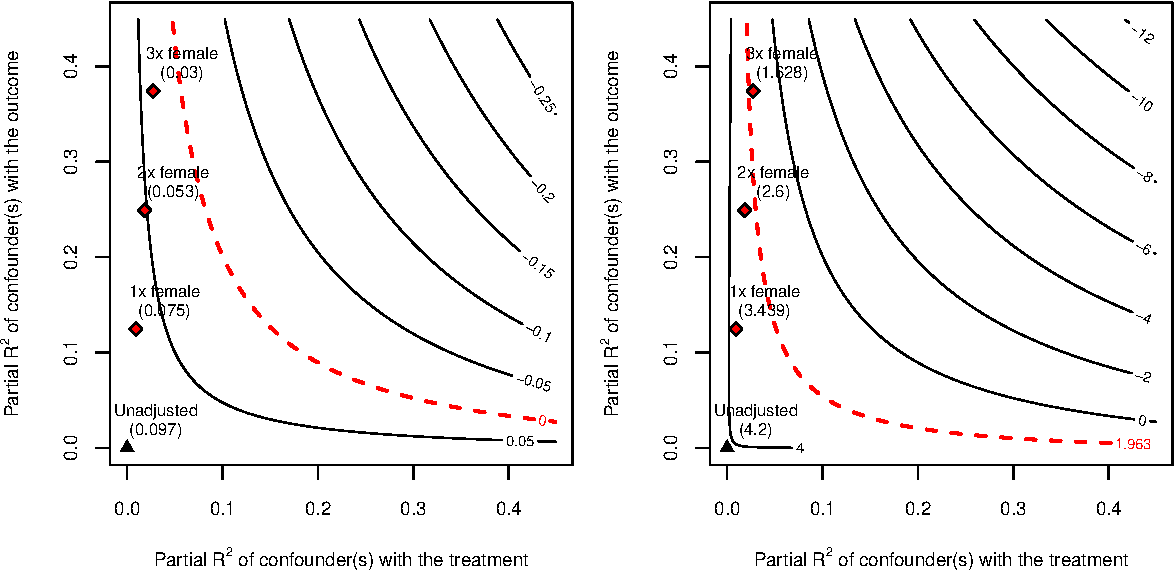
\includegraphics[width=420px,height=210px]{jss_sensemakr_files/figure-latex/both_plots_real-1} 

}

\caption{\label{fig:darfur_contours}Sensitivity contour plots of point estimate (left) and t-value (right)}\label{fig:both_plots_real}
\end{figure}
\end{CodeChunk}

The resulting plot is shown in the right of Figure
\ref{fig:darfur_contours}. At the 5\% significance level, the null
hypothesis of zero effect would still be rejected given confounders once
or twice as strong as \texttt{female}. However, while the point-estimate
remains positive, accounting for sampling uncertainty now means that the
null hypothesis of zero effect \emph{would not} be rejected with the
inclusion of a confounder three times as strong as \texttt{female}.

\hypertarget{sensitivity-plots-of-extreme-scenarios}{%
\subsubsection{Sensitivity plots of extreme
scenarios}\label{sensitivity-plots-of-extreme-scenarios}}

Sometimes researchers may be better equipped to make plausibility
judgments about the strength of determinants of the treatment assignment
mechanism, and have less knowledge about the determinants of the
outcome. In those cases, sensitivity plots using \emph{extreme
scenarios} are a useful option. These are produced with the option
\texttt{type\ =\ extreme}. Here one assumes confounding explains
\textbf{all} or some large fraction of the residual variance of the
outcome, then vary how strongly such confounding is hypothetically
related to the treatment, to see how this affects the resulting point
estimate.

\begin{CodeChunk}

\begin{CodeInput}
R> plot(darfur.sensitivity, type = "extreme")
\end{CodeInput}
\begin{figure}[t]

{\centering 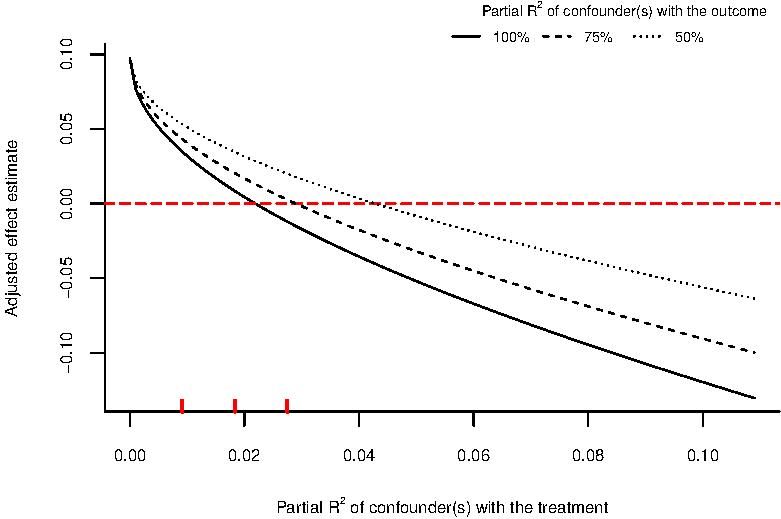
\includegraphics[width=350px,height=250px]{jss_sensemakr_files/figure-latex/darfur_extreme-1} 

}

\caption{\label{fig:extreme}Sensitivity analysis to extreme scenarios.}\label{fig:darfur_extreme}
\end{figure}
\end{CodeChunk}

Figure \ref{fig:extreme} shows the result. By default these plots
consider confounding that explains 100\%, 75\%, and 50\% of variation in
the residual outcome,producing three separate curves for each scenario.
This is equivalent to setting the argument
\texttt{r2yz.dx\ =\ c(1,\ .75,\ .5)}. The bounds on the strength of
association of a confounder once, twice or three times as strongly
associated with the treatment as \texttt{female} are shown as red ticks
in the horizontal axis. As the plot shows, even in the most extreme case
(\(R^2_{Y\sim Z| {\bf X}, D}=100\%\)), confounders would need to be more
than twice as strongly associated with the treatment as \texttt{female}
to fully explain away the point estimate. Moving to the scenarios
\(R^2_{Y\sim Z| {\bf X}, D}=75\%\) and
\(R^2_{Y\sim Z| {\bf X}, D}=50\%\), confounders would need to be more
than three times as strongly associated with the treatment as
\texttt{female} to fully explain away the point estimate.

\hypertarget{lecturing}{%
\subsection{A disciplined discussion about
confounding}\label{lecturing}}

Having demonstrated the basic functionality of the package, we end this
section by recalling some important caveats on intepretation that apply
to any sensitivity analyses. Readers may refer to
\citet{cinelli:jrssb2019} for further discussion. The results computed
by \texttt{sensemakr()} tell us what we need to be prepared to believe
in order to sustain that a given conclusion is not due to confounding.
In particular, the results of the sensitivity analysis performed here
show that, to explain all the observed estimated effect, even in a worst
case scenario where the unobserved confounder explains all residual
variation of the outcome, this unobserved confounder would need to be
more than twice as strongly associated with the treatment as the
covariate \texttt{female}. This is a \emph{true quantitative statement}
that describes the strength of confounding needed to overturn the
research conclusions.

To counter a common misconception, we emphasize that such an analysis
says nothing about whether such a confounder does or does not exist. The
role of sensitivity analysis is, instead, to \emph{discipline the
discussion} regarding the causal interpretation of the effect estimate.
In particular,

\begin{enumerate}
\def\labelenumi{\arabic{enumi}.}
\item
  A causal interpretation of the research conclusion may be defended by
  articulating that a confounder with such strength is unlikely to
  exist. For instance, one could argue that, given the way injuries (the
  ``treatment'') occurred, the scope for targeting particular types of
  individuals was quite limited; aircraft dropped makeshift and unguided
  bombs and other objects over villages, and militia raided without
  concern for who they would attack---the only known major exception to
  this, due to sexual assaults, was targeting gender, which is also one
  of the most visually apparent characteristics of an individual.
\item
  Likewise, similar grounds are required to persuasively dismiss a
  causal interpretation of the result. There are requirements, in terms
  of (relative) strength, that the hypothesized unobserved confounders
  need to meet in order to be problematic. For instance, helpful
  skepticism must articulate why a confounder that explains at least
  more than twice of the variation of the treatment assignment than the
  covariate \texttt{female} is plausible. Otherwise, the putative
  confounder cannot logically account for all the observed association,
  even in an extreme scenario.
\end{enumerate}

Robustness to confounding is thus claimed to the extent one agrees with
the arguments in 1 (which rely on domain knowledge about attacks in
Darfur), while a result can be deemed fragile insofar as alternative
stories meeting the requirements in 2 can be offered. Sensitivity
analyses should not be used to obviate discussions about confouding by
engaging in automatic procedures; rather, they should stimulate a more
disciplined, quantitative argument about confounding, in which such
statements are made and debated.

\hypertarget{r-adv}{%
\section{sensemakr for R: advanced use}\label{r-adv}}

The functionality demonstrated in the previous section will suffice for
most users, most of the time. Sometimes, however, more flexibility will
be needed, and can be obtained by employing additional functions of
\pkg{sensemakr} for \proglang{R}. The functions most likely to be called
upon can be divided into the following categories:

\begin{itemize}
\item
  \emph{functions for computing the bias, adjusted estimates and
  standard errors:} these comprise, among others, the functions
  \texttt{bias()}, \texttt{adjusted\_estimate()},
  \texttt{adjusted\_se()} and \texttt{adjusted\_t()}. They take as input
  the original (unadjusted) estimate (in the form of a linear model or
  numeric values) and a pair of sensitivity parameters (the partial
  \(R^2\) of the omitted variable with the treatment and the outcome),
  and return the new quantity adjusted for omitted variable bias.
\item
  \emph{functions for computing sensitivity statistics}: these comprise,
  among others, the functions \texttt{partial\_r2()},
  \texttt{robustness\_value()}, and \texttt{sensitivity\_stats()}. These
  functions compute sensitivity statistics suited for routine reporting,
  as proposed in \citet{cinelli:jrssb2019}. They take as input the
  original (unadjusted) estimate (in the form of a linear model or
  numeric values), and return the corresponding sensitivity statistic.
\item
  \emph{sensitivity plots}: These functions provide direct access to
  sensitivity contour plots, \texttt{ovb\_contour\_plot()}, and
  sensitivity plots of extreme scenarios, \texttt{ovb\_extreme\_plot()},
  for customization. There is also a convenience function
  \texttt{add\_bound\_to\_contour()} which facilitates the placement of
  user computed bounds on contour plots. All plot functions return
  invisibly the data needed to replicate the plot, so users that prefer
  fully customized plots can also easily do so. The default options for
  plots work best with width and height around 4 to 5 inches.
\item
  \emph{bounding functions}: these functions compute bounds on the
  strength of confounding ``k times'' as strong as certain observed
  covariates. The main high level function is \texttt{ovb\_bounds()},
  and there is also the auxiliary function
  \texttt{ovb\_partial\_r2\_bound()}.
\end{itemize}

We demonstrate the use of these functions below through examples chosen
to illustrate important features of sensitivity analysis.

\hypertarget{informal}{%
\subsection{Formal versus informal benchmarking: customizing
bounds}\label{informal}}

Informal ``benchmarking'' procedures have been suggested as aids to
interpretation for numerous sensitivy analyses. These approaches are
usually described as revealing how an unobserved confounder \(Z\) ``not
unlike'' some observed covariate \(X_j\) would alter the results of a
study
\citep{imbens2003sensitivity, blackwell2013selection, hosman2010sensitivity, carnegie:jree2016, dorie2016flexible, hong:jebs2018}.
As shown in \cite{cinelli:jrssb2019}, these informal proposals may lead
users to erroneous conclusions, even when they have correct knowledge of
how unobserved confounders compare to observed covariates. Here we
replicate Section 6.1 of \citet{cinelli:jrssb2019} using
\pkg{sensemakr}, and provide a numerical example that illustrates the
potential for misleading results from informal benchmarking. This
example also demonstrates advanced usage of the package, including how
to construct sensitivity contour plots with customized bounds.

\hypertarget{data-and-model}{%
\subsubsection{Data and model}\label{data-and-model}}

We begin by simulating the data generating process which will be used in
our example, as given by Equations \ref{eq:naive_first} to
\ref{eq:naive_last} below. Here we have a treatment variable \(D\), an
outcome variable \(Y\), one observed confounder \(X\), and one
\emph{unobserved} confounder \(Z\). All disturbance variables \(U\) are
standardized mutually independent normals. Note that, in reality, the
treatment \(D\) has \emph{no causal effect} on the outcome \(Y\).

\paragraph{Model 1:}

\begin{align}
Z &= U_{z}\label{eq:naive_first}\\
X &= U_{x}\\
D &= X + Z + U_d\\
Y &= X + Z + U_y \label{eq:naive_last}
\end{align}

Also note that, in this model: (i) the unobserved confounder \(Z\) is
independent of \(X\); and, (ii) the unobserved confounder \(Z\) is
\emph{exactly like} \(X\) in terms of its strength of association with
the treatment and the outcome. The code below creates a sample of size
100 of this data generating process. We use the function
\texttt{resid\_maker()} to make sure the residuals are standardized and
orthogonal, thus all properties that we describe here hold exactly even
with finite sample size.

\begin{CodeChunk}

\begin{CodeInput}
R> n <- 100
R> X <- scale(rnorm(n))
R> Z <- resid_maker(n, X) 
R> D <- X + Z + resid_maker(n, cbind(X, Z)) 
R> Y <- X + Z + resid_maker(n, cbind(X, Z, D))
\end{CodeInput}
\end{CodeChunk}

In this example, the investigator knows she need to adjust for the
confounder \(Z\) but, unfortunately, does not observe \(Z\). Therefore,
she is forced to fit the restricted linear model adjusting for \(X\)
only.

\begin{CodeChunk}

\begin{CodeInput}
R> model.ydx <- lm(Y ~ D + X) 
\end{CodeInput}
\end{CodeChunk}

Results from this regression are shown in the first column of Table
\ref{tab:naive}, showing a large and statistically significant
coefficient estimate \(X\).

\begin{table}
\centering


\begin{tabular}{@{\extracolsep{5pt}}lcc} 
\\[-1.8ex]\hline 
\hline \\[-1.8ex] 
 & \multicolumn{2}{c}{\textit{Dependent variable:}} \\ 
\cline{2-3} 
\\[-1.8ex] & \multicolumn{2}{c}{Y} \\ 
 & Restricted OLS & Full OLS \\ 
\\[-1.8ex] & (1) & (2)\\ 
\hline \\[-1.8ex] 
 D & 0.500$^{***}$ & 0.000 \\ 
  & (0.088) & (0.102) \\ 
  & & \\ 
 X & 0.500$^{***}$ & 1.000$^{***}$ \\ 
  & (0.152) & (0.144) \\ 
  & & \\ 
 Z &  & 1.000$^{***}$ \\ 
  &  & (0.144) \\ 
  & & \\ 
\hline \\[-1.8ex] 
Observations & 100 & 100 \\ 
R$^{2}$ & 0.500 & 0.667 \\ 
Adjusted R$^{2}$ & 0.490 & 0.656 \\ 
Residual Std. Error & 1.240 (df = 97) & 1.020 (df = 96) \\ 
F Statistic & 48.500$^{***}$ (df = 2; 97) & 64.000$^{***}$ (df = 3; 96) \\ 
\hline 
\hline \\[-1.8ex] 
\textit{Note:}  & \multicolumn{2}{r}{$^{*}$p$<$0.1; $^{**}$p$<$0.05; $^{***}$p$<$0.01} \\ 
\end{tabular} 

\caption{First column: results of the restricted regression adusting for $X$ only. Second column: results of the full regression adusting for $X$ and $Z$.}
\label{tab:naive}
\end{table}

\hypertarget{formal-benchmarks}{%
\subsubsection{Formal benchmarks}\label{formal-benchmarks}}

Let us suppose the investigator \emph{correctly} knows that: (i) \(Z\)
and \(X\) have the same strength of association with \(D\) and \(Y\);
and, (ii) \(Z\) is independent of \(X\). How can she leverage this
information to understand how much bias a confounder \(Z\) ``not
unlike'' \(X\) could cause? As we have seen in Section \ref{bounds},
using Equation \ref{eq:bounds} it is possible to obtain valid bounds on
the amount of confounding caused by an unobserved \(Z\) as strongly
associated with the treatment \(D\) and with the outcome \(Y\) as the
observed covariate \(X\).

Separately from the main \texttt{sensemakr()} function, these bounds can
be computed with the function \texttt{ovb\_bounds()}. In this function
one needs to specify the linear model being used
(\texttt{model\ =\ model.ydx}), the treatment of interest
(\texttt{treatment\ =\ "D"}), the observed variable used for
benchmarking (\texttt{benchmark\_covariates\ =\ "X"}), and how many
times stronger \(Z\) is in explaining treatment (\texttt{kd\ =\ 1}) and
outcome (\texttt{ky\ =\ 1}) variation, as compared to the benchmark
variable \(X\).

\begin{CodeChunk}

\begin{CodeInput}
R> formal_bound <- ovb_bounds(model = model.ydx, 
R+                            treatment = "D", 
R+                            benchmark_covariates = "X", 
R+                            kd = 1, 
R+                            ky = 1)
\end{CodeInput}
\end{CodeChunk}

We can now inspect the output of \texttt{ovb\_bounds()}.

\begin{CodeChunk}

\begin{CodeInput}
R> formal_bound[1:6]
\end{CodeInput}
\end{CodeChunk}

\begin{CodeChunk}

\begin{CodeOutput}
  bound_label r2dz.x r2yz.dx treatment adjusted_estimate adjusted_se
1        1x X    0.5   0.333         D                 0       0.102
\end{CodeOutput}
\end{CodeChunk}

As we can see, the results of the bounding procedure correctly shows us
that, an unobserved confounder \(Z\) that is truly ``not unlike \(X\)''
would: (1) explain 50\% of the residual variation of the treatment and
33\% of the residual variation of the outcome; (2) bring the point
estimate exactly to zero; and, (3) bring the standard error to 0.102.
This is precisely what one obtains when running the full regression
model adjusting for \emph{both} \(X\) and \(Z\), as shown in the second
column of Table \ref{tab:naive}.

\hypertarget{informal-benchmarks}{%
\subsubsection{Informal benchmarks}\label{informal-benchmarks}}

We now demonstrate an ``informal benchmark'' to show its dangers.
Computing the bias due to the omission of \(Z\) requires two sensitivity
parameters: its partial \(R^2\) with the treatment \(D\) and its partial
\(R^2\) with the outcome \(Y\). Informal approaches follow from the
intuition that we can simply take the observed partial \(R^2\) of \(X\)
with \(D\) and \(Y\) found directly from regressions for the treatment
and the outcome, respectively. Unfortunately, as formalized in
\cite{cinelli:jrssb2019}, these observed associations are themselves
affected by the omission of the omitted variable, making naive
comparisons potentially misleading.

What happens if we nevertheless attempt to use those observed statistics
for benchmarking? To compute the informal benchmarks, we first need to
obtain the observed partial \(R^2\) of \(X\) with the outcome \(Y\).
This can be done using the \texttt{partial\_r2()} function of
\texttt{sensemakr} in the \texttt{model.ydx} regression.

\begin{CodeChunk}

\begin{CodeInput}
R> r2yx.d <- partial_r2(model.ydx, covariates = "X")
\end{CodeInput}
\end{CodeChunk}

We next need to obtain the partial \(R^2\) of \(X\) with the treatment
\(D\). For that, we need to fit a new regression of the treatment \(D\)
on the observed covariate \(X\) here denoted by \texttt{model.dx}.

\begin{CodeChunk}

\begin{CodeInput}
R> model.dx <- lm(D ~ X)
R> r2dx   <- partial_r2(model.dx, covariates = "X")
\end{CodeInput}
\end{CodeChunk}

We then determine what would be the implied adjusted estimate due to an
unobserved confounder \(Z\) with this pair of partial \(R^2\) values.
This can be computed using the \texttt{adjusted\_estimate()} function.

\begin{CodeChunk}

\begin{CodeInput}
R> informal_adjusted_estimate <- adjusted_estimate(model     = model.ydx, 
R+                                                 treatment = "D", 
R+                                                 r2dz.x    = r2dx, 
R+                                                 r2yz.dx   = r2yx.d)
\end{CodeInput}
\end{CodeChunk}

Let us now compare those informal benchmarks with the formal bounds. To
prepare, we first plot sensitivity contours with the function
\texttt{ovb\_contour\_plot()}. Next, we add the informal benchmark to
the contours, using the numeric method of the function
\texttt{add\_bound\_to\_contour()}. Finally, we use
\texttt{add\_bound\_to\_contour()} again to add the previously computed
formal bounds.

\begin{CodeChunk}

\begin{CodeInput}
R> # draws sensitivity contours
R> ovb_contour_plot(model = model.ydx,  
R+                  treatment = "D", 
R+                  lim = .6)
R> 
R> # adds informal benchmark 
R> add_bound_to_contour(r2dz.x = r2dx, 
R+                      r2yz.dx = r2yx.d, 
R+                      bound_value = informal_adjusted_estimate,
R+                      bound_label = "Informal benchmark")
R> 
R> # adds formal bound
R> add_bound_to_contour(bounds = formal_bound, 
R+                      bound_label = "Formal bound")
\end{CodeInput}
\begin{figure}[!tp]

{\centering 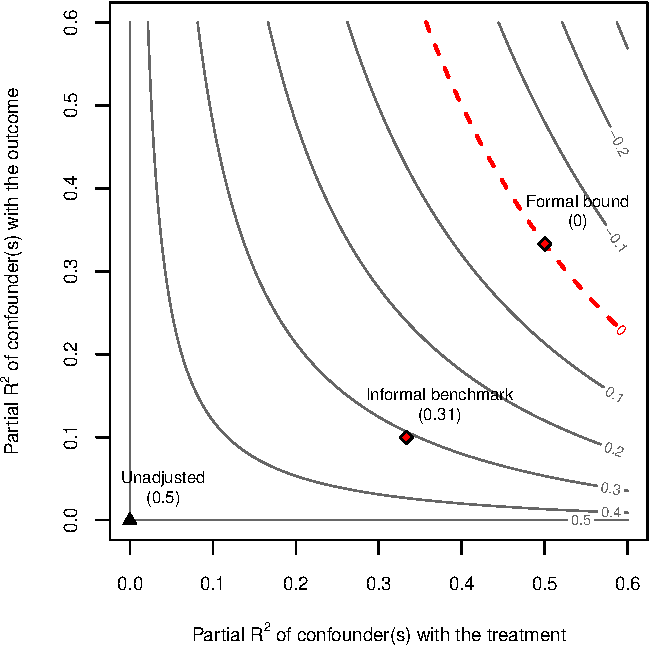
\includegraphics[width=250px,height=250px]{jss_sensemakr_files/figure-latex/informal_benchmark_plot-1} 

}

\caption{\label{fig:naive_benchmarking}Informal benchmarking \emph{versus} proper bounds.}\label{fig:informal_benchmark_plot}
\end{figure}
\end{CodeChunk}

Note how the results from informal benchmarking are misleading: even
though \(Z\) and \(X\) are exactly alike in their roles, the informal
benchmark point is still far from zero, which would suggest that an
unobserved confounder \(Z\) ``not unlike'' \(X\) is unable to explain
away the observed effect, when in fact we know it would, as shown in
Table \ref{tab:naive}. This incorrect conclusion occurs \emph{despite}
the investigator \emph{correctly} assuming both that: (i) \(Z\) and
\(X\) have the same strength of association with \(D\) and \(Y\); and,
(ii) \(Z\) is independent of \(X\). Therefore, we do not recommend using
informal benchmarks for sensitivity analysis, and suggest empirical
researchers to use formal approaches such as the ones provided with
\texttt{ovb\_bounds()}. For further details and discussion, we point
readers to Sections 4.4 and 6.1 of \citet{cinelli:jrssb2019}.

\hypertarget{print}{%
\subsection{Assessing the sensitivity of existing regression
results}\label{print}}

We conclude this section by demonstrating how to replicate Section
\ref{r-basic} using only the statistics found in the regression table
along with the individual functions available in the package.

\hypertarget{sensitivity-statistics}{%
\subsubsection{Sensitivity statistics}\label{sensitivity-statistics}}

The robustness value and partial \(R^2\) are key sensitivity statistics,
useful for standardized sensitivity analyses reporting. Beyond the main
\texttt{sensemakr()} function, these statistics can be computed directly
by the user with the functions \code{robustness_value()} and
\code{partial_r2()}. With a fitted \code{lm} model in hand, the most
convenient way to compute the RV and partial \(R^2\) is by employing the
\code{lm} methods for these functions, as in

\begin{CodeChunk}

\begin{CodeInput}
R> robustness_value(model = darfur.model, covariates = "directlyharmed")
R> partial_r2(model = darfur.model, covariates = "directlyharmed")
\end{CodeInput}
\end{CodeChunk}

\noindent However, when one does not have access to the data in order to
run this model, simple summary statistics such as: (i) the point
estimate for the \texttt{directlyharmed} (0.097); (ii) its estimtaed
standard error (\texttt{0.023}); and, (ii) the degrees of freedom of the
regression (\texttt{783}) are sufficient to compute the RV and partial
\(R^2\).

\begin{CodeChunk}

\begin{CodeInput}
R> robustness_value(t_statistic = 0.097/0.023, dof = 783)
R> partial_r2(t_statistic = 0.097/0.023, dof = 783)
\end{CodeInput}
\end{CodeChunk}

The convenience function \code{sensitivity_stats()} also computes all
sensitivity statistics for a regression coefficient of interest and
returns them in a \code{data.frame}.

\hypertarget{plotting-functions}{%
\subsubsection{Plotting functions}\label{plotting-functions}}

All plotting functions can be called directly with \texttt{lm} objects
or numerical data. For example, the code below uses the function
\texttt{ovb\_contour\_plot()} to replicate Figure
\ref{fig:darfur_contours} (without the bounds) using only the summary
statistics of Table \ref{tab:darfur_ols}.

\begin{CodeChunk}

\begin{CodeInput}
R> ovb_contour_plot(estimate = 0.097, se = 0.023, dof = 783)
R> ovb_contour_plot(estimate = 0.097, se = 0.023, dof = 783, 
R>                  sensitivity.of = "t-value")
\end{CodeInput}
\end{CodeChunk}

The extreme scenario plots (as in Figure \ref{fig:extreme}) can also be
reproduced from summary statistics using the function
\texttt{ovb\_extreme\_plot()},

\begin{CodeChunk}

\begin{CodeInput}
R> ovb_extreme_plot(estimate = 0.097, se = 0.023, dof = 783)
\end{CodeInput}
\end{CodeChunk}

All plotting functions return (invisibly) the data needed to reproduce
them, allowing users to create their own plots if they prefer.

\hypertarget{adjusted-estimates-standard-errors-and-t-values}{%
\subsubsection{Adjusted estimates, standard errors and
t-values}\label{adjusted-estimates-standard-errors-and-t-values}}

These functions allow users to compute the adjusted estimates given
different postulated degrees of confounding. For instance, suppose a
researcher has reasons to believe a confounder explains 10\% of the
residual variance of the treatment and 15\% of the residual variance of
the outcome. If the underlying data are not available, the investigator
can still compute the adjustd estimate and t-value that one would have
obtained in the full regression adjusting for such confounder.

\begin{CodeChunk}

\begin{CodeInput}
R> adjusted_estimate(estimate = 0.097, se = 0.023, dof = 783, 
R+                   r2dz.x = .1, r2yz.dx = 0.15)
\end{CodeInput}

\begin{CodeOutput}
[1] 0.0139
\end{CodeOutput}

\begin{CodeInput}
R> adjusted_t(estimate = 0.097, se = 0.023, dof = 783, 
R+            r2dz.x = .1, r2yz.dx = 0.15)
\end{CodeInput}

\begin{CodeOutput}
[1] 0.622
\end{CodeOutput}
\end{CodeChunk}

The computation shows that this confounder is not strong enough to bring
the estimate to zero, but it is sufficient to bring the t-value below
the usual 5\% signifiance threshold of 1.96.

\hypertarget{computing-bounds-from-summary-statistics}{%
\subsubsection{Computing bounds from summary
statistics}\label{computing-bounds-from-summary-statistics}}

Finally, we show how users can compute bounds on the strength of
confounding using only summary statistics, if the paper also provides a
\emph{treatment} regression table, i.e., a regression of the treatment
on the observed covariates. Such regressions are sometimes shown in
published works as part of efforts to describe the ``determinants'' of
the treatment, or as ``balance tests'' in which the investigator
assesses whether observed covariates predict treatment assigment. For
the Darfur example, this regression is shown in Table
\ref{tab:treat_reg}.

\begin{table}
\centering

\begin{tabular}{@{\extracolsep{5pt}}lc} 
\\[-1.8ex]\hline 
\hline \\[-1.8ex] 
 & \multicolumn{1}{c}{\textit{Dependent variable:}} \\ 
\cline{2-2} 
\\[-1.8ex] & directlyharmed \\ 
\hline \\[-1.8ex] 
 female & $-$0.097$^{***}$ \\ 
  & (0.036) \\ 
  & \\ 
\hline \\[-1.8ex] 
Observations & 1,276 \\ 
R$^{2}$ & 0.426 \\ 
Adjusted R$^{2}$ & 0.066 \\ 
Residual Std. Error & 0.476 (df = 784) \\ 
F Statistic & 1.180$^{**}$ (df = 491; 784) \\ 
\hline 
\hline \\[-1.8ex] 
\textit{Note:}  & \multicolumn{1}{r}{$^{*}$p$<$0.1; $^{**}$p$<$0.05; $^{***}$p$<$0.01} \\ 
\end{tabular} 

\caption{Treatment regression for the Darfur example. Due to space, only the results for \texttt{female} are shown, which will be used for benchmarking.}
\label{tab:treat_reg}
\end{table}

Using the results of Tables \ref{tab:darfur_ols} and \ref{tab:treat_reg}
we can compute the bounds on confounding 1, 2 and 3 times as strong as
\texttt{female}, as we have done before. First we compute the partial
\(R^2\) of \texttt{female} with the treatment and the outcome

\begin{CodeChunk}

\begin{CodeInput}
R> r2yxj.dx <- partial_r2(t_statistic = -0.232/0.024, dof = 783)
R> r2dxj.x <- partial_r2(t_statistic = -0.097/0.036, dof = 783)
\end{CodeInput}
\end{CodeChunk}

Next, we compute the bounds on the partial \(R^2\) of the unobserved
confounder using the \texttt{ovb\_partial\_r2\_bound()} function.

\begin{CodeChunk}

\begin{CodeInput}
R> bounds <- ovb_partial_r2_bound(r2dxj.x = r2dxj.x,
R+                                r2yxj.dx = r2yxj.dx,
R+                                kd = 1:3,
R+                                ky = 1:3,
R+                                bound_label = paste(1:3, "x", "female"))
\end{CodeInput}
\end{CodeChunk}

Finally, the \texttt{adjusted\_estimate()} function computes the
estimates implied by such hypothetical confounders.

\begin{CodeChunk}

\begin{CodeInput}
R> bound.values <- adjusted_estimate(estimate = 0.0973,
R+                                   se = 0.0232,
R+                                   dof = 783,
R+                                   r2dz.x = bounds$r2dz.x,
R+                                   r2yz.dx = bounds$r2yz.dx)
\end{CodeInput}
\end{CodeChunk}

This information along with the numeric methods for the plot functions,
allow us to reproduce the contour plots of Figure
\ref{fig:darfur_contours} using only summary statistics. Note that,
since we are performing all calculations manually, appropriate limits of
the plot area need to be set by the user.

\begin{CodeChunk}

\begin{CodeInput}
R> ovb_contour_plot(estimate = 0.0973, se = 0.0232, dof = 783, lim = 0.45)
R> add_bound_to_contour(bounds, bound_value = bound.values)
\end{CodeInput}
\end{CodeChunk}

\hypertarget{stata}{%
\section{sensemakr for Stata}\label{stata}}

For \proglang{Stata} users, we have also developed a homonymous package
\pkg{sensemakr}.

\pkg{sensemakr} for \textbackslash proglang\{Stata{]} is available for
download on SCC\ldots{}

It also comes with the \texttt{darfur} data (?).

In this section, we demonstrate how to replicate the analysis of Section
\ref{r-basic} using the \textbackslash proglang\{Stata{]} implementation
of sensemakr. The main function of the \pkg{Stata} package is
\texttt{sensemakr}\ldots{}

\hypertarget{final-remarks}{%
\section{Final Remarks}\label{final-remarks}}

In this article we have demonstrated how to perform sensitivity analysis
to unobserved confounding using the \proglang{R} and \proglang{Stata}
packages \pkg{sensemakr}.

These packages can help making sensitivity analyisis routine and
standardized.

\renewcommand\refname{References}
\bibliography{sensemakr.bib}


\end{document}

